\chapter{Spatial disparity-coherent watermarking}
\markright{Spatial disparity-coherent watermarking}
\label{spa}
\phantomsection
%\addcontentsline{toc}{chapter}{Spatial watermarking}



As said in the previous chapter, a number of works focused on how to incorporate depth information into the perceptual shaping process of the embedded watermark.\newline This process allows to achive disparity-coherence and makes sure that a physical point of the captured scene carries the same watermark sample regardless of where it appears in the left and right view.\newline

This process brings two advantages: it produces stereoscopic views more in line with reality, therefore yields less visual discomfort; and it is expected to have superior robustness against view synthesis.\newline

\section{Prior work} 

A prior work that is based on the disparity-coherent technique is the one carried on by Doerr et al in "Blind Detection for Disparity-Coherent
Stereo Video Watermarking" \cite{DOER2}.\newline
The watermark strategy  assumes that the key-seeded reference watermark pattern $w_{K}\textasciitilde N(0, 1)$ is embedded spatially in the left view and subsequently transferred to the right one.\newline
The watermark embedding and detection operations for the left view are therefore given by the conventional spread-spectrum equations:\newline
$$f_{l}^{w} = f_{l}+\alpha w_{K}$$
$$\rho(f_{l}+\epsilon\alpha w_{K},w_{K})= \frac{1}{wh}\sum_{x,y}(f_{l}(x,y)+\epsilon\alpha w_{K}(x,y))w_{K}(x,y)\approx\epsilon\alpha $$
where the superscript w indicates watermarked quantities, the subscript l (resp. r ) denotes quantities related to the left (resp. right) view, $\alpha > 0$ is the embedding strength, and w is normally distributed with zero mean and unit variance.\newline
The embedding strenght used in \cite{DOER2} to keep the embedding distortion imperceptible is $\alpha = 3$.\newline 

For the right view, the watermarking equation is the same, except that the watermark pattern $w_{K}$ is warped according to the depth information prior to insertion.

$$\forall(x,y) \in [1:w][1:h] f_{r}^{w}(x,y) = f_{r}(x,y)+\alpha w_{K}(x+d(x,y),y) = f_{r}+\alpha w_{K}^{d}(x,y) $$

The watermark detection on the right view relies on the computation of a horizontal cross-correlation array.\newline
$$\rho (f_{r}+\epsilon\alpha w_{K}^{d},w_{K}^{s})\approx\epsilon\alpha D_{s} $$
$$ \rho = \epsilon\alpha [D_{smin},..,D_{0},..,S_{smax}]$$
where $D_{s}$ is the proportion of pixels whose disparity value is exactly equal to s.\newline
The correlation array is then mapped into a scalar value in order to compare it with a threshold and to decide whether the tested content contains the watermark. Authors proposed three possible mapping functions:

$$\rho_{max}= \max_{s}\rho[s] $$
$$ \sum_{s}\rho[s] $$
$$ \sum_{|rho[s]|>\tau_{\rho}}|\rho[s]| $$

\section{ Gaussian-noise disparity-coherent watermarking} 

Based on the described technique, we propose a new spatial watermarking technique. \newline
For the spatial watermark its been taken under consideration the insertion of a Gaussian-noise reference watermark in an additive way.\newline
As in Doerr et al, the left view is processed in the conventional way, with spred-spectrum equations (riferimento all'equazione); the watermark is then warped according to the disparity value and inserted in the right view (rif all'eq), taking under consideration that the occluded zones shoudn't be processed.\newline
The added pattern and the reference images have the same size, so it should be noted that the warping process will generate a loss of marked pixel, due to the baseline's lenght.\newline
\begin{figure}[h!]
\centering
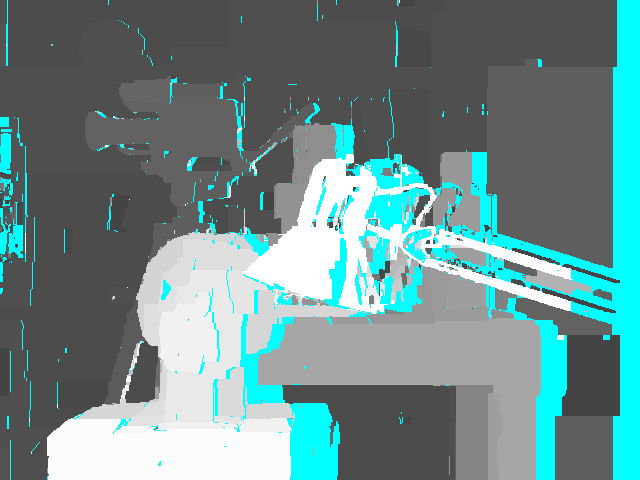
\includegraphics[width=0.5\textwidth]{./img/disp_left_to_right.png}
\caption{\small{Disparity left-to-right computed with KZ}}
\label{fig:kzdisplr}
\end{figure}
Since the disparity map and the occclusion map are usually not available, it needs to be estimated through the KZ algorithm, before the warping process.\newline
The embedding strenght is $\alpha=1$; it should be noted that this baseline watermarking framework could be enriched with conventional add-ons, e.g. perceptually modulate the embedding strength to better accommodate for the human visual system or canceling host interference for improved detection statistics.\newline

In the detection process, it has been used a conventional correlation-based detector for the left view (ref to eq).\newline 
On the other hand to detect the watermark in the right view two differet correlation-based strategies are proposed:
in the first strategy we computed the correlation value between the non-distorted watermark and the right view warped according to the right-to-left disparity, this way the priviously warped watermark is restored, even if there will be discontinuities due the occluded zones. In formula:
$$\rho((f_{r}+\epsilon\alpha w_{K}^{*})^{*},w_{K})= \frac{1}{wh}\sum_{x,y}(f_{r}(x,y)+\epsilon\alpha w_{K}^{*}(x,y))^{*}w_{K}(x,y)\approx\epsilon\alpha $$
where the superscript * indicates the warped mark/image.\newline

The second strategy is again a simple correlation-based detector, but the correlation value is computed between the right view and the warped watermark instead of the original one, based on the fact that the right view should contain this, rather than the reference pattern and that the reciever can compute the disparity map thats needed to warp the mark and perform the detection.

$$\rho(f_{r}+\epsilon\alpha w_{K}^{*},w_{K}^{*})= \frac{1}{wh}\sum_{x,y}(f_{r}(x,y)+\epsilon\alpha w_{K}^{*}(x,y))w_{K}^{*}(x,y)\approx\epsilon\alpha $$

To illustrates the performance of the binary classifier system as its discrimination threshold is varied it has been drawn the corresponding ROC curve.\newline  The ROC curve is a representation of the sensitivity as a function of fall-out.\newline  The curve is created by plotting the true positive rate (TPR) against the false positive rate (FPR) at various threshold settings.\newline The true-positive rate is also known as sensitivity and the false-positive rate is also known as the fall-out.\newline  

\begin{figure}[h!]
\centering
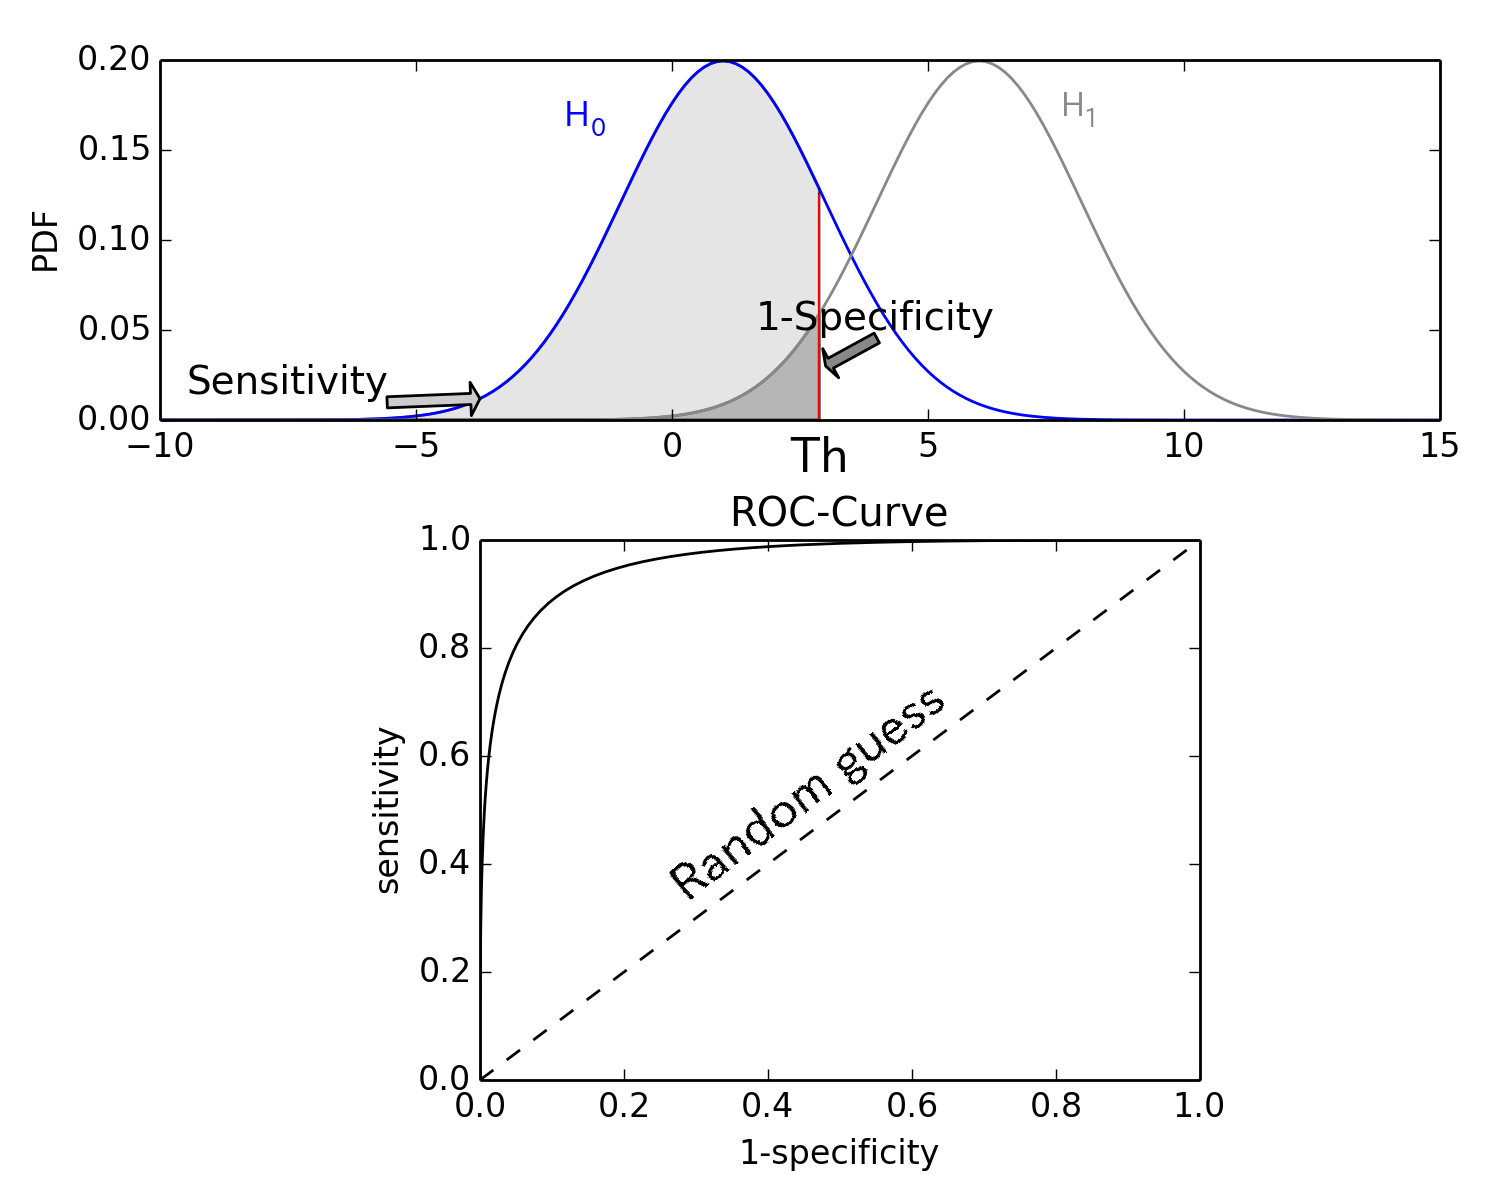
\includegraphics[width=0.7\textwidth]{./img/roc.png}
\caption{\small{Top: Probability density functions for two distributions. Bottom: corresponding ROC-curve.}}
\label{fig:roc}
\end{figure}

\begin{figure}[h!]
\centering
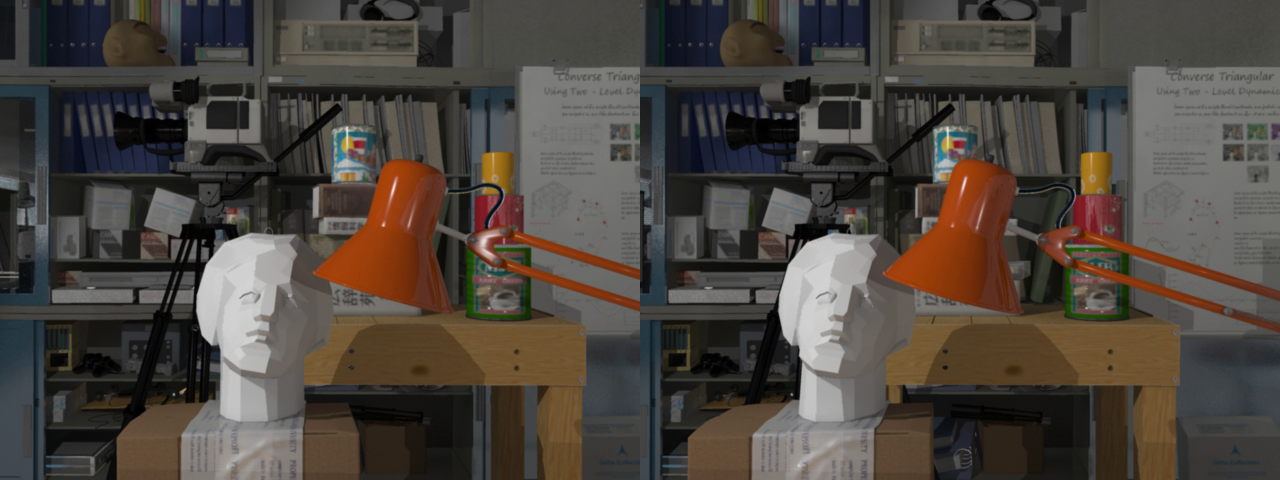
\includegraphics[width=1\textwidth]{./img/marked_1_gauss.png}
\caption{\small{Stereo image marked with spatial algorithm with power equal to 1.}}
\label{fig:gauss1}
\end{figure}
\begin{figure}[h!]
\centering
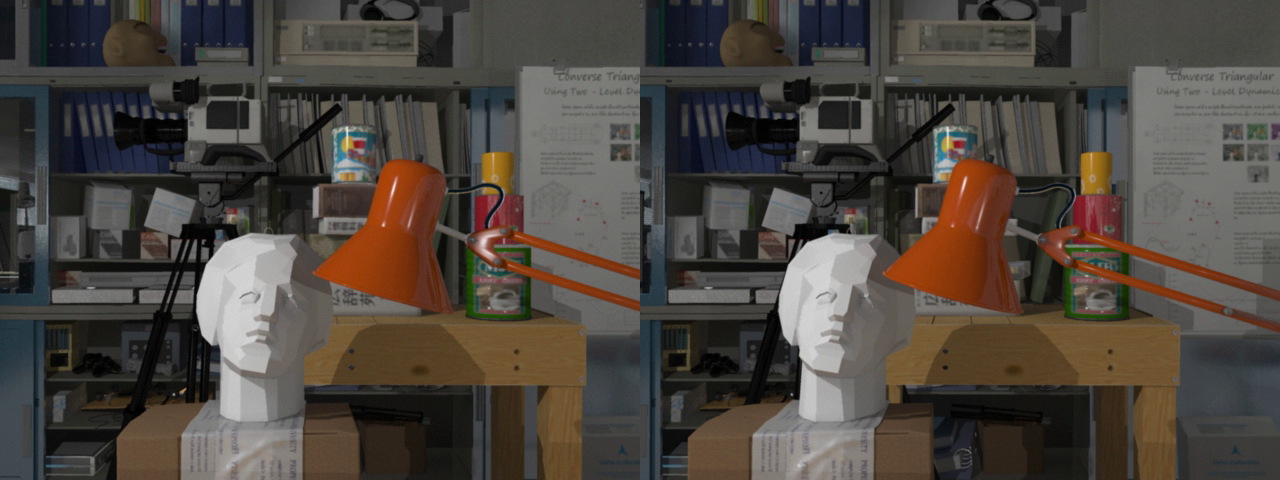
\includegraphics[width=1\textwidth]{./img/marked_3_gauss.png}
\caption{\small{Stereo image marked with spatial algorithm with power equal to 1}}
\label{fig:gauss3}
\end{figure}
  
As said before the disparity-coherent watermarking have the ability to detect the embedded watermark in synthetized views: to performe the detection on a random right view, that might be synthetized, the detector will need to calculate the disparity map between the analyzed view and the recieved left, and warp it accordingly, to recompose the original watermark.\newline 
There is then a tight bond between the watermarking process and the evaluation of the disparity maps; with the graph-cuts algorithm it's possible to compute accurate maps and to know the occluded zones.
